\documentclass{article}

\usepackage[english]{babel}
\usepackage[letterpaper,top=2cm,bottom=2cm,left=3cm,right=3cm,marginparwidth=1.75cm]{geometry}
\usepackage{amsmath}
\usepackage{booktabs}
\usepackage{caption}
\usepackage{graphicx}
\usepackage{makecell}
\usepackage{pdflscape}


\newcommand*{\PathToOutput}{../output/}


\begin{document}

\title{Evaporating Liquidity - Replication Report}

\author{
    Ruilong Guo,
    Sifei Zhao,
    Zhiyuan Liu,
    Junhan Fu
}


\maketitle


\section{Introduction}
This project replicates Table 1 and 2 in Evaporating Liquidity\cite{nagel}. The author
shows that the returns of short-term reversal strategies are generated by liquidity 
provision, and therefore are highly predictable by the VIX index. The author also 
found that reversal strategies on not only individual stocks but also industry portfolios 
produce high returns, especially during periods of high VIX.

The author constructs the reversal strategy by averaging the returns of five substrategies
that weight stocks (or industries) proportional to the negative of market-adjusted returns
on days $t-1$ to $t-5$.
\begin{equation}
    w_{it}^R = -\left( \frac{1}{2} \sum_{i=1}^{N} \left| R_{it-1} - R_{mt-1} \right| \right)^{-1} \left( R_{it-1} - R_{mt-1} \right),
\end{equation}
where $R_{mt-1} = \frac{1}{N}\sum_{i=1}^N R_{it-1}$ is the equal-weighted market return.
Table 1 reports the summary statistics of the reversal strategies on individual stocks 
and industry portfolios. For individual stocks, the returns are calculated based on 
end-of-day transaction prices and quote midpoints.

Table 2 reports the results of the following predictive regression
\begin{equation}
    L_t^R = a + bVIX_{t-5} + c'g_{t-5} + e_t,
\end{equation}
where $L_t^R$ is the return of the reversal strategy. $VIX_{t-5}$ is the VIX index lagged
by 5 days, divided by $\sqrt{250}$. $g_{t-5}$ is a vector of control variables, including 
pre-decimalization dummy (takes a value of one prior to April 9, 2001 and a value of zero 
thereafter) and market return.

This project replicates these two tables using the same sample range as the original
paper (from January 1998 to December 2010). We also provide the updated tables using
data from January 1998 to December 2023.
\section{Data Description}

\begin{landscape}
\begin{table}
    \centering
    \caption*{Table: Additional Summary Statistics of Reversal Strategy Returns}

    \raggedright
    \small
    Apart from the original statistical analysis of reversal strategy provided by 
    the paper, we create a new version of performance matrix which includes VaR(0.05), 
    CVaR(0.05), max drawdown, and other drawdown-based strategy perfomance, and we also 
    add CRSP value weighted index as the benchmark to evaluate the performance of reversal strategies. 

    Compared to the CRSP value weighted index, the reversal strategy based on individual 
    stocks tends to have much higher annualized mean return and lower annualized volatility, 
    which cause a way higher annualized sharpe ratio. The mean return of industry reversal 
    strategy is a little bit lower than the banchmark, but it has lower volatility 
    with higher sharpe ratio.

    With regard to max drawdown, the transact price based individual reversal strategy 
    is the best(-4.38\%) among all the reversal strategies(quote-midpoints: -7.70\%, 
    industry: -13.90\%) and the CRSP index(-57.18\%). That strategy dropped form the 
    peak on 2009-10-22 after the period of financial crisis. And it only used 7 days to 
    recover the lose since the peak, while the industry reversal strategy took 433 days 
    to recover and CRSP value weighted index didn't recover to the peak.
    \medskip

    \centering
    \begin{tabular}{lllll}
\toprule
 & Transact. prices & Quote-midpoints & Industry portfolio & CRSP Value Weighted Index \\
\midrule
Annualized Mean Return(\%) & 76.97 & 48.23 & 4.02 & 7.86 \\
Annualzied Volatility(\%) & 8.94 & 10.60 & 8.85 & 19.65 \\
Annualized Sharpe Ratio & 8.61 & 4.55 & 0.45 & 0.40 \\
Skewness & 3.01 & 3.55 & 0.77 & -0.27 \\
Kurtosis & 38.46 & 49.69 & 14.60 & 12.01 \\
VaR (0.05)(\%) & -0.33 & -0.61 & -0.74 & -1.92 \\
CVaR (0.05)(\%) & -0.67 & -1.02 & -1.22 & -2.96 \\
Max Drawdown(\%) & -4.38 & -7.70 & -13.90 & -57.18 \\
Peak & 2000-04-11 & 2001-07-13 & 1998-04-09 & 2007-10-09 \\
Bottom & 2000-04-14 & 2001-09-21 & 1998-10-08 & 2009-03-09 \\
Recovery Date & 2000-04-18 & 2001-10-24 & 1999-06-16 & 2013-03-08 \\
Duration (days) & 7 & 103 & 433 & 1977 \\
\bottomrule
\end{tabular}

\end{table}

\begin{figure}
    \centering
    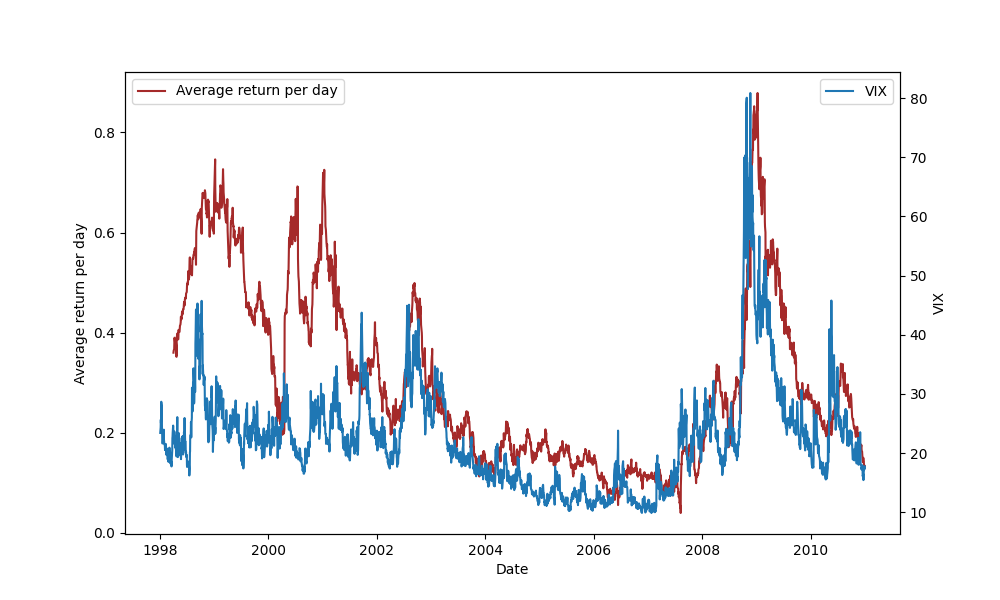
\includegraphics[width=0.8\textwidth]{\PathToOutput/reversal_strategy_vix.png}
    \caption{Reversal Strategy and VIX}

    \raggedright
    \medskip
    \small 
    This figure shows the three-month moving average return of the reversal strategy 
    and VIX index across 1998 to 2010. The blue curve(VIX index) has a pre-trend of 
    the red curve(3-month MA return of reversal strategy), which presents a key finding 
    of the paper that the VIX index has a power to predict the reversal strategy return.

    During the LTCM crisis in 1998 and  Nasdaq decline in 2000, the reversal strategy 
    return increased with VIX increasing. From then until 2007, returns declined steadily
    to less than 0.2\% per day, but during the financial crisis, they surged, surpassing 
    levels seen during the LTCM crisis. The figure illustrates a strong correlation 
    between the time variation in the reversal strategy's return and the VIX index. 
    Since the financial crisis began in 2007, the returns of the reversal strategy 
    and the VIX have closely tracked each other.
\end{figure}

\end{landscape}

\begin{table}
    \centering
    \caption*{Table 1:  Summary Statistics of Reversal Strategy Returns}

    \begin{tabular}{lccc}
    \toprule
    & Indiv. stock reversal & Indiv. stock reversal & Industry \\
    & Transact. prices & Quote-midpoints & Portfolio reversal \\
    \midrule
    \multicolumn{4}{c}{Panel A: Raw Returns} \\
    \midrule
    Mean return(\% per day) & 0.30 & 0.18 & 0.02 \\
    Std.dev.(\% per day) & 0.56 & 0.61 & 0.52 \\
    Skewness & 3.02 & 2.74 & 1.06 \\
    Kurtosis & 38.21 & 40.50 & 17.93 \\
    Worst day return(\%) & -3.88 & -4.76 & -3.93 \\
    Worst 3-month return(\%) & 2.56 & -2.13 & -9.28 \\
    Beta & 0.11 & 0.11 & 0.09 \\
    Annualized Sharpe Ratio & 8.44 & 4.50 & 0.56 \\
    \midrule
    \multicolumn{4}{c}{Panel B: Returns hedged for conditional market factor exposure} \\
    \midrule
    Mean return(\% per day) & 0.29 & 0.17 & 0.01 \\
    Std.dev.(\% per day) & 0.48 & 0.54 & 0.47 \\
    Skewness & 2.45 & 2.26 & 0.88 \\
    Kurtosis & 31.26 & 34.51 & 15.97 \\
    Worst day return(\%) & -2.26 & -3.92 & -3.12 \\
    Worst 3-month return(\%) & 2.27 & -1.28 & -7.97 \\
    Beta & 0.00 & 0.00 & 0.00 \\
    Annualized Sharpe Ratio & 9.58 & 4.91 & 0.44 \\
    \bottomrule
    \end{tabular}
\end{table}


\begin{table}
    \centering
    \caption*{Table 1:  Summary Statistics of Reversal Strategy Returns (Replicated)}

    \begin{tabular}{lccc}
\toprule
& Indiv. stock reversal & Indiv. stock reversal & Industry \\
& Transact. prices & Quote-midpoints & Portfolio reversal \\
\midrule
\multicolumn{4}{c}{Panel A: Raw Returns} \\
\midrule
Mean return(\% per day) & 0.31 & 0.19 & 0.02 \\
Std.dev.(\% per day) & 0.56 & 0.67 & 0.56 \\
Skewness & 3.01 & 3.58 & 0.77 \\
Kurtosis & 38.46 & 50.26 & 14.60 \\
Worst day return(\%) & -3.84 & -4.54 & -3.70 \\
Worst 3-month return(\%) & 2.51 & -2.72 & -12.17 \\
Beta & 0.11 & 0.09 & 0.10 \\
Annualized Sharpe Ratio & 8.61 & 4.54 & 0.45 \\
\midrule
\multicolumn{4}{c}{Panel B: Returns hedged for conditional market factor exposure} \\
\midrule
Mean return(\% per day) & 0.30 & 0.19 & 0.01 \\
Std.dev.(\% per day) & 0.54 & 0.65 & 0.54 \\
Skewness & 3.02 & 3.84 & 0.65 \\
Kurtosis & 39.00 & 55.98 & 12.20 \\
Worst day return(\%) & -3.05 & -3.96 & -3.31 \\
Worst 3-month return(\%) & 2.07 & -2.02 & -9.18 \\
Beta & 0.00 & 0.00 & 0.00 \\
Annualized Sharpe Ratio & 8.87 & 4.58 & 0.38 \\
\bottomrule
\end{tabular}
\end{table}


\begin{table}
    \centering
    \caption*{Table 1:  Summary Statistics of Reversal Strategy Returns (Updated)}

    \begin{tabular}{lccc}
\toprule
& Indiv. stock reversal & Indiv. stock reversal & Industry \\
& Transact. prices & Quote-midpoints & Portfolio reversal \\
\midrule
\multicolumn{4}{c}{Panel A: Raw Returns} \\
\midrule
Mean return(\% per day) & 0.23 & 0.16 & 0.01 \\
Std.dev.(\% per day) & 0.67 & 0.77 & 0.52 \\
Skewness & -0.51 & 4.97 & 0.70 \\
Kurtosis & 48.95 & 136.49 & 14.54 \\
Worst day return(\%) & -12.44 & -7.50 & -3.70 \\
Worst 3-month return(\%) & -7.53 & -9.62 & -12.17 \\
Beta & 0.12 & 0.10 & 0.09 \\
Annualized Sharpe Ratio & 5.39 & 3.29 & 0.32 \\
\midrule
\multicolumn{4}{c}{Panel B: Returns hedged for conditional market factor exposure} \\
\midrule
Mean return(\% per day) & 0.22 & 0.16 & 0.01 \\
Std.dev.(\% per day) & 0.65 & 0.76 & 0.50 \\
Skewness & -0.72 & 5.39 & 0.64 \\
Kurtosis & 52.57 & 151.89 & 12.62 \\
Worst day return(\%) & -12.47 & -7.49 & -3.30 \\
Worst 3-month return(\%) & -5.39 & -9.79 & -10.05 \\
Beta & -0.00 & -0.00 & -0.00 \\
Annualized Sharpe Ratio & 5.44 & 3.27 & 0.22 \\
\bottomrule
\end{tabular}
\end{table}


\begin{landscape}
\begin{table}
    \centering
    \caption*{Table 2: Predicting Reversal Strategy Returns with VIX}
    
    \small Original Table 2 from the paper.
    \medskip

    \begin{tabular}{lcccccccccccc}
\toprule
& \multicolumn{4}{c}{\makecell{Individual stocks\\Transaction-price returns}} & \multicolumn{4}{c}{\makecell{Individual stocks\\Quote-midpoint returns}} & \multicolumn{4}{c}{\makecell{Industry\\portfolios}} \\
& \multicolumn{3}{c}{Daily} & Monthly & \multicolumn{3}{c}{Daily} & Monthly & \multicolumn{3}{c}{Daily} & Monthly \\
& (1) & (2) & (3) & (4) & (5) & (6) & (7) & (8) & (9) & (10) & (11) & (12) \\
\midrule
Intercept & -0.03 & -0.05 & -0.02 & 0.02 & -0.06 & -0.07 & -0.04 & -0.01 & -0.08 & -0.09 & -0.06 & -0.05 \\
& (0.03) & (0.02) & (0.02) & (0.02) & (0.03) & (0.03) & (0.03) & (0.02) & (0.02) & (0.02) & (0.02) & (0.01) \\
VIX & 0.22 & 0.20 & 0.18 & 0.15 & 0.16 & 0.16 & 0.13 & 0.10 & 0.07 & 0.07 & 0.05 & 0.04 \\
& (0.02) & (0.02) & (0.02) & (0.01) & (0.02) & (0.02) & (0.02) & (0.02) & (0.02) & (0.02) & (0.02) & (0.01) \\
Pre-decim. & & 0.22 & 0.22 & 0.23 & & 0.08 & 0.09 & 0.09 & & 0.00 & 0.01 & 0.01 \\
& & (0.03) & (0.03) & (0.03) & & (0.03) & (0.03) & (0.03) & & (0.02) & (0.02) & (0.02) \\
$R_M$ & & & -0.60 & -0.03 & & & -0.59 & -0.16 & & & -0.42 & -0.05 \\
& & & (0.19) & (0.26) & & & (0.21) & (0.28) & & & (0.17) & (0.16) \\
Adj. $R^2$ & 0.07 & 0.11 & 0.11 & 0.56 & 0.03 & 0.03 & 0.04 & 0.25 & 0.01 & 0.01 & 0.01 & 0.07 \\
\bottomrule
\end{tabular}

\end{table}


\begin{table}
    \centering
    \caption*{Table 2: Predicting Reversal Strategy Returns with VIX (Replicated)}

    \raggedright
    \small Replicated Table 2, which uses the same sample range as the original (from 
    January 1998 to December 2010). 
    It has been verified that coefficients of predictor variables in the replicated result
    have the same sign with the original result. The coefficients of replicated result are
    within the 99.7\% confidence interval of the original result.
    \medskip

    \centering
    \begin{tabular}{lcccccccccccc}
\toprule
 & \multicolumn{4}{c}{\makecell{Individual stocks\\Transaction-price returns}} & \multicolumn{4}{c}{\makecell{Individual stocks\\Quote-midpoint returns}} & \multicolumn{4}{c}{\makecell{Industry\\portfolios}} \\
 & \multicolumn{3}{c}{Daily} & Monthly & \multicolumn{3}{c}{Daily} & Monthly & \multicolumn{3}{c}{Daily} & Monthly \\
 & (1) & (2) & (3) & (4) & (5) & (6) & (7) & (8) & (9) & (10) & (11) & (12) \\
\midrule
Intercept & -0.06 & -0.09 & -0.06 & -0.01 & -0.06 & -0.07 & -0.03 & 0.00 & -0.10 & -0.10 & -0.07 & -0.04 \\
 & (0.03) & (0.02) & (0.03) & (0.02) & (0.03) & (0.03) & (0.04) & (0.03) & (0.03) & (0.03) & (0.03) & (0.02) \\
VIX & 0.25 & 0.23 & 0.21 & 0.18 & 0.18 & 0.17 & 0.14 & 0.11 & 0.08 & 0.08 & 0.06 & 0.04 \\
 & (0.02) & (0.02) & (0.02) & (0.01) & (0.03) & (0.03) & (0.03) & (0.02) & (0.02) & (0.02) & (0.02) & (0.01) \\
Pre-decim. &  & 0.23 & 0.24 & 0.25 &  & 0.11 & 0.11 & 0.12 &  & 0.01 & 0.01 & 0.02 \\
 &  & (0.03) & (0.03) & (0.03) &  & (0.03) & (0.03) & (0.03) &  & (0.02) & (0.02) & (0.02) \\
$R_M$ &  &  & -0.45 & 0.10 &  &  & -0.78 & -0.28 &  &  & -0.57 & -0.21 \\
 &  &  & (0.19) & (0.23) &  &  & (0.23) & (0.26) &  &  & (0.21) & (0.16) \\
Adj. $R^2$ & 0.07 & 0.10 & 0.10 & 0.65 & 0.02 & 0.03 & 0.03 & 0.27 & 0.01 & 0.01 & 0.01 & 0.07 \\
\bottomrule
\end{tabular}

\end{table}

\begin{table}
    \centering
    \caption*{Table 2: Predicting Reversal Strategy Returns with VIX (Updated)}

    \small Updated Table 2, using data from January 1998 to December 2023.
    The results are consistent.
    \medskip

    \begin{tabular}{lcccccccccccc}
\toprule
 & \multicolumn{4}{c}{\makecell{Individual stocks\\Transaction-price returns}} & \multicolumn{4}{c}{\makecell{Individual stocks\\Quote-midpoint returns}} & \multicolumn{4}{c}{\makecell{Industry\\portfolios}} \\
 & \multicolumn{3}{c}{Daily} & Monthly & \multicolumn{3}{c}{Daily} & Monthly & \multicolumn{3}{c}{Daily} & Monthly \\
 & (1) & (2) & (3) & (4) & (5) & (6) & (7) & (8) & (9) & (10) & (11) & (12) \\
\midrule
Intercept & -0.08 & -0.08 & -0.05 & -0.01 & -0.09 & -0.09 & -0.06 & -0.02 & -0.09 & -0.09 & -0.07 & -0.06 \\
 & (0.02) & (0.03) & (0.02) & (0.02) & (0.03) & (0.03) & (0.03) & (0.03) & (0.02) & (0.02) & (0.02) & (0.02) \\
VIX & 0.24 & 0.21 & 0.19 & 0.15 & 0.19 & 0.18 & 0.17 & 0.12 & 0.08 & 0.08 & 0.07 & 0.05 \\
 & (0.02) & (0.02) & (0.02) & (0.02) & (0.02) & (0.03) & (0.02) & (0.03) & (0.02) & (0.02) & (0.02) & (0.01) \\
Pre-decim. &  & 0.26 & 0.27 & 0.28 &  & 0.09 & 0.10 & 0.12 &  & 0.00 & 0.00 & 0.01 \\
 &  & (0.03) & (0.03) & (0.03) &  & (0.03) & (0.03) & (0.03) &  & (0.02) & (0.02) & (0.02) \\
$R_M$ &  &  & -0.39 & 0.03 &  &  & -0.47 & -0.04 &  &  & -0.24 & -0.03 \\
 &  &  & (0.17) & (0.18) &  &  & (0.23) & (0.26) &  &  & (0.16) & (0.13) \\
Adj. $R^2$ & 0.04 & 0.05 & 0.05 & 0.53 & 0.02 & 0.02 & 0.02 & 0.19 & 0.01 & 0.01 & 0.01 & 0.08 \\
\bottomrule
\end{tabular}

\end{table}

\end{landscape}

\newpage
\bibliographystyle{jpe}
\bibliography{bibliography.bib}

\end{document}